\subsection{Iterative Agent Trajectories Accumulate Quality Issues}\label{sec:iteraitve-degrade}

\begin{figure}[ht]
    \centering
    \makebox[\textwidth][c]{%
        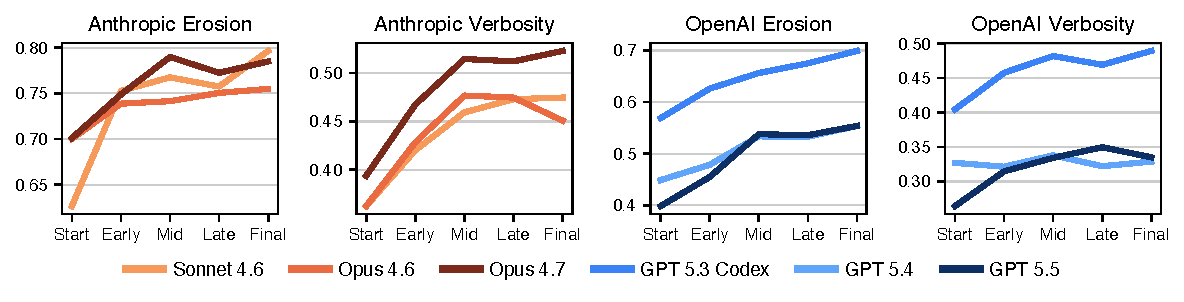
\includegraphics[width=1.15\textwidth]{figures/complexity_sign_flip.pdf}%
    }
    \caption{\textbf{Models from both frontier labs produce similar degradation trends as the problem progresses}. Erosion and verbosity across problem progress for six representative models.}
    \label{fig:accumulation-results}
\end{figure}

\autoref{fig:accumulation-results} highlights the changes in quality throughout frontier models' trajectories on problems. Across all settings, structural erosion increases in \erosionPctIncreasing\% of trajectories, verbosity in \vfTrajIncPct\%. The average number of functions with at least 10 cyclomatic complexity rises from \erosionHighCcCountFirstMean{} to \erosionHighCcCountLastMean{} and mean maximum CC from \newErosionFirstCcMaxMean{} to \newErosionLastCcMaxMean{}. This behavior would be invisible without iterative evaluation.

Opus~4.7's \texttt{main()} on \href{https://www.scbench.ai/problems/forge}{\texttt{forge}} grows \erosionForgeMainCcMultiplier$\times$ in CC across \erosionForgeNumCkpts{} checkpoints, from \erosionForgeMainLinesFirst{} to \erosionForgeMainLinesLast{} lines. The $\ckpt{1}$ \texttt{argparse} call, shown in \autoref{lst:erosion-main-cp1}, is replaced by a manual flag loop in which seven flags each get an identical pair of \verb|--X val|/\verb|--X=val| branches and no helper is extracted (\autoref{lst:erosion-main-cp8}). The accumulation over time highlights the key failure mode.

Verbosity behaves similarly to erosion. Structural duplication grows \vfCloneGrowthPct\% while AST-grep violation density grows only \vfAstOverallGrowth\%, reflecting the rewriting of existing code rather than fresh rule violations. \textbf{Iterative evaluation makes accumulation visible; small structural choices are amplified by iteration rather than absorbed.}
